% Options for packages loaded elsewhere
\PassOptionsToPackage{unicode}{hyperref}
\PassOptionsToPackage{hyphens}{url}
%
\documentclass[
]{article}
\usepackage{amsmath,amssymb}
\usepackage{lmodern}
\usepackage{iftex}
\ifPDFTeX
  \usepackage[T1]{fontenc}
  \usepackage[utf8]{inputenc}
  \usepackage{textcomp} % provide euro and other symbols
\else % if luatex or xetex
  \usepackage{unicode-math}
  \defaultfontfeatures{Scale=MatchLowercase}
  \defaultfontfeatures[\rmfamily]{Ligatures=TeX,Scale=1}
\fi
% Use upquote if available, for straight quotes in verbatim environments
\IfFileExists{upquote.sty}{\usepackage{upquote}}{}
\IfFileExists{microtype.sty}{% use microtype if available
  \usepackage[]{microtype}
  \UseMicrotypeSet[protrusion]{basicmath} % disable protrusion for tt fonts
}{}
\makeatletter
\@ifundefined{KOMAClassName}{% if non-KOMA class
  \IfFileExists{parskip.sty}{%
    \usepackage{parskip}
  }{% else
    \setlength{\parindent}{0pt}
    \setlength{\parskip}{6pt plus 2pt minus 1pt}}
}{% if KOMA class
  \KOMAoptions{parskip=half}}
\makeatother
\usepackage{xcolor}
\usepackage[margin=1in]{geometry}
\usepackage{graphicx}
\makeatletter
\def\maxwidth{\ifdim\Gin@nat@width>\linewidth\linewidth\else\Gin@nat@width\fi}
\def\maxheight{\ifdim\Gin@nat@height>\textheight\textheight\else\Gin@nat@height\fi}
\makeatother
% Scale images if necessary, so that they will not overflow the page
% margins by default, and it is still possible to overwrite the defaults
% using explicit options in \includegraphics[width, height, ...]{}
\setkeys{Gin}{width=\maxwidth,height=\maxheight,keepaspectratio}
% Set default figure placement to htbp
\makeatletter
\def\fps@figure{htbp}
\makeatother
\setlength{\emergencystretch}{3em} % prevent overfull lines
\providecommand{\tightlist}{%
  \setlength{\itemsep}{0pt}\setlength{\parskip}{0pt}}
\setcounter{secnumdepth}{-\maxdimen} % remove section numbering
\colorlet{mycolor}{red}
\usepackage{tcolorbox}
\renewtcolorbox{quote}{}
\ifLuaTeX
  \usepackage{selnolig}  % disable illegal ligatures
\fi
\IfFileExists{bookmark.sty}{\usepackage{bookmark}}{\usepackage{hyperref}}
\IfFileExists{xurl.sty}{\usepackage{xurl}}{} % add URL line breaks if available
\urlstyle{same} % disable monospaced font for URLs
\hypersetup{
  hidelinks,
  pdfcreator={LaTeX via pandoc}}

\author{}
\date{\vspace{-2.5em}}

\begin{document}

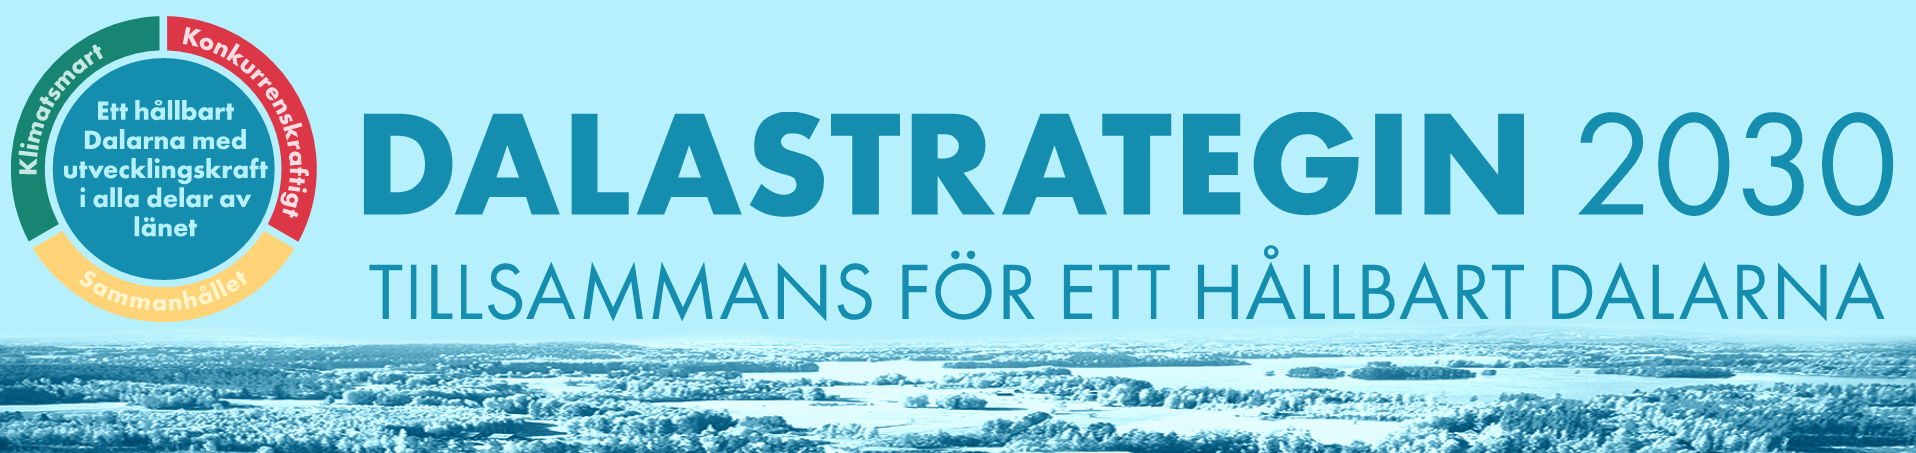
\includegraphics{G:/skript/projekt/uppfoljning_rus/Bilder/dalaheader.png}

\hypertarget{introduktion}{%
\section{Introduktion}\label{introduktion}}

Dalarna står inför stora samhällsutmaningar som i många stycken delas
med övriga Sverige, Europa och världen. I juni 2021 antog
Regionfullmäktige i Dalarna en ny regional utvecklingsstrategi:
Dalastrategin - Tillsammans för ett hållbart Dalarna. Strategin är ett
stöd och en språngbräda i arbetet med att rusta Dalarna för att möta
framtidsutmaningarna och göra dem till möjligheter. Dalastrategin är
indelad i tre olika målområden som kopplar an till de olika
dimensionerna av hållbarhet - miljömässig, ekonomisk och social
hållbarhet: ett klimatsmart Dalarna, ett konkurrenskraftigt Dalarna och
ett sammanhållet Dalarna.

En princip för genomförandet av Dalastrategin är ett kunskapsbaserat
arbetssätt, vilken bland annat innefattar uppföljning, utvärdering och
ett kontinuerligt lärande. En central del av uppföljningsarbetet är de
indikatorer som kopplas till respektive målområde och den här rapporten
är en del av den årliga uppföljningen av utvecklingen i länet baserat på
dessa indikatorer.

Klimatsmart

Konkurrenskraftigt

Sammanhållet

{Utsläpp av klimatpåverkande växthusgaser }

{Representation i chefspositioner }

{Trångboddhet }

{Energiproduktion }

{Ginikoefficient }

{Boendetyper }

{Energieffektivitet }

{Internationaliseringsgrad }

{Tillgång till service och tjänster }

{Insamlat hushållsavfall (kg/person) }

{Branschbredd och branschstruktur* }

{Tillgänglighet till vård* }

{Avfall/BRP }

{Nyföretagande }

{Deltagande i det civila samhället }

{Laddinfrastruktur för fordon* }

{Andel av transporter via olika trafikslag* }

{Andel av hushåll som har tillgång till bredband }

{Andel kollektivt resande }

{Tillgänglighet (restid) till arbetsplatser/skolor* }

{Valdeltagande }

{Självförsörjningsgrad av energi och livsmedel }

{Infrastrukturinvesteringar }

{Tillit till andra människor }

{Andel hektar formellt skyddad produktiv skogsmark }

{Matchningsgrad }

{Digitalt deltagande* }

Arealen betesmark och areal med särskilt höga biologiska värden*

{Andel sysselsatta }

{Andel invånare i ekonomiskt utsatta hushåll }

{ }

{Långtidsarbetslöshet }

{Andel unga som upplever att de är delaktiga i sin kommun}

{ }

{Andel unga som inom fyra år fullföljer gymnasieutbildning}

{Självskattad hälsa }

{ }

{Andel högskoleutbildade i befolkningen }

{ }

{ }

{Etableringstid för nyanlända }

{ }

{ }

{Investeringar i FoU }

{ }

*Datainsamling pågår och indikatorn är under utveckling

\hypertarget{ett-klimatsmart-dalarna}{%
\section{Ett klimatsmart Dalarna}\label{ett-klimatsmart-dalarna}}

Ett klimatsmart Dalarna är ett resurseffektivt Dalarna utan
klimatpåverkande utsläpp. Resande sker på ett enkelt och miljömässigt
hållbart sätt. I ett klimatsmart Dalarna är samhällets robusthet och
resiliens vid klimatförändringar god.

Den miljömässiga dimensionen i regional utveckling handlar om att
säkerställa att ekosystemen fortsätter leverera de tjänster som
samhället är beroende av. Genom att gå före i en miljömässigt hållbar
omställning gynnas innovationer och regionalt företagande när regionala
lösningar bidrar till att lösa globala problem. Det är också så vi
skapar goda livsmiljöer och levnadsvillkor.

\hypertarget{utsluxe4pp-av-klimatpuxe5verkande-vuxe4xthusgaser}{%
\subsection{Utsläpp av klimatpåverkande
växthusgaser}\label{utsluxe4pp-av-klimatpuxe5verkande-vuxe4xthusgaser}}

2017 antogs ett långsiktigt nationellt mål om att Sverige ska vara
klimatneutralt år 2045. Detta är definierat som minst 85 procent lägre
växthusgasutsläpp inom landets gränser jämfört med år 1990. Målet
innebär i princip att alla sektorer och verksamheter behöver vara
fossilfria år 2045. De nationella målen bidrar till det internationella
Parisavtalet samt det europeiska målet om 85-90 procent minskning av
utsläppen till år 2050.

Utsläppen i Dalarna visar på en positiv trend där utsläppen av
växthusgaser har minskat över tid. Även om detta är en utveckling i rätt
riktning kommer det att krävas en ännu snabbare minskningstakt för att
kunna uppnå målen på både nationell nivå och för att svara upp mot
ambitionerna i Dalastrategin. I ett nationellt perspektiv ligger Dalarna
högre än riksgenomsnittet sett till utsläpp per person, trots en
minskning från knappt 7,5 till drygt 5,5 ton/invånare. Likt övriga
Sverige är det industrin och transporterna i länet som står för den
största andelen utsläpp av växthusgaser.

\begin{center}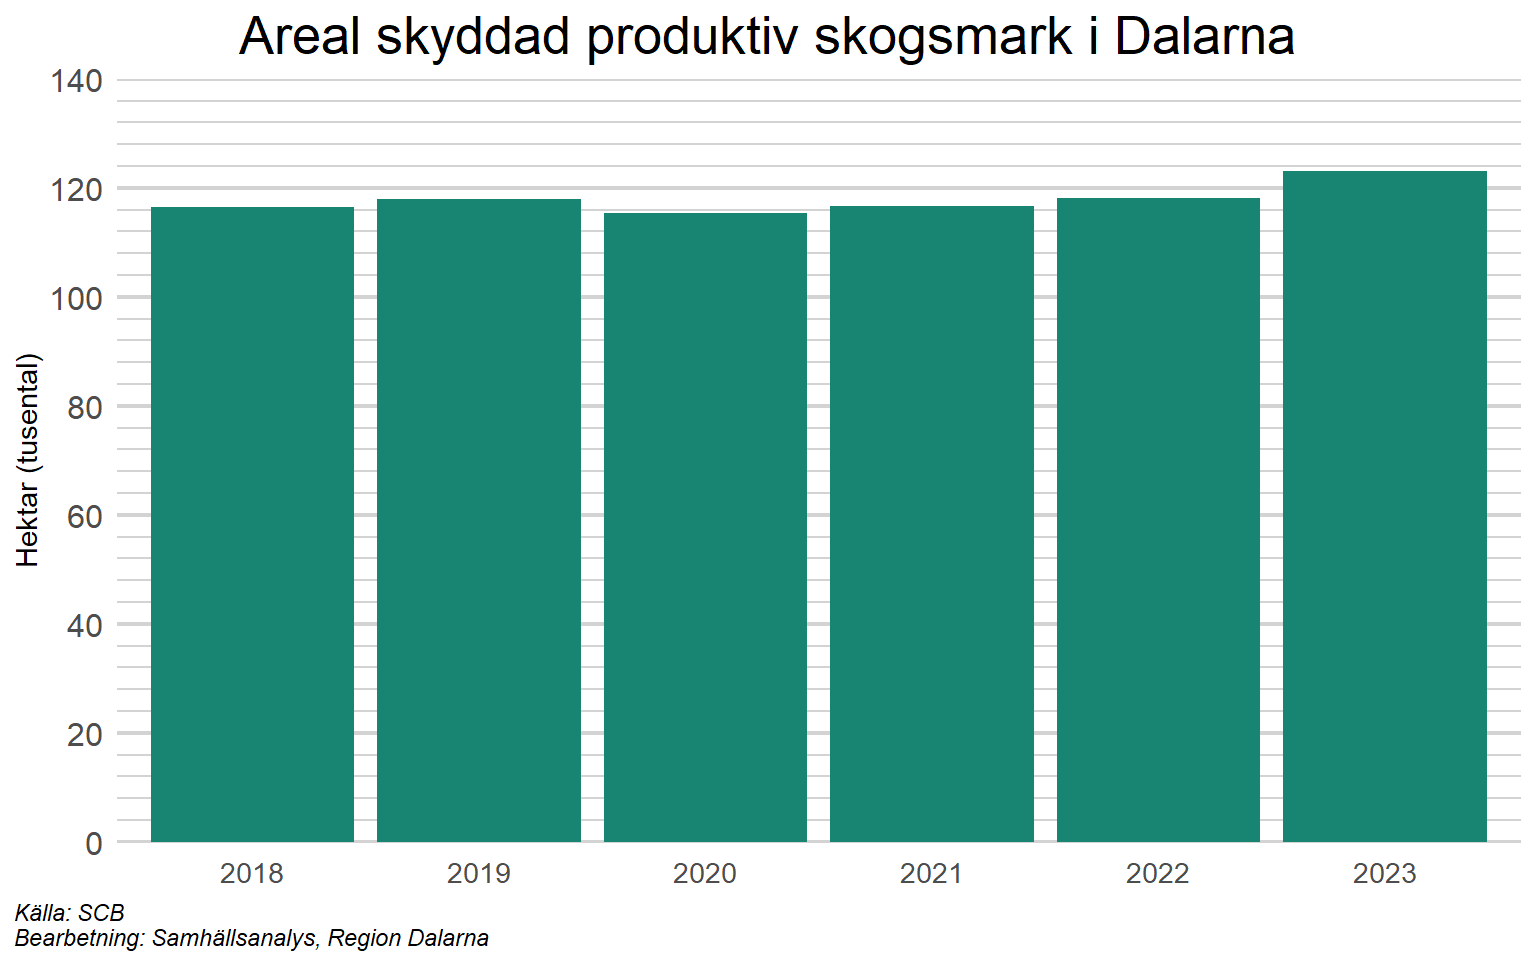
\includegraphics{dalarapport_files/figure-latex/unnamed-chunk-4-1} \end{center}

\begin{center}\includegraphics{dalarapport_files/figure-latex/unnamed-chunk-4-2} \end{center}

\newpage

\hypertarget{energiproduktion}{%
\subsection{Energiproduktion}\label{energiproduktion}}

I Dalastrategin konstateras det att en god tillgång till hållbar energi
är avgörande för näringslivets och hela samhällets
omställningskapacitet. En ökad produktion av förnybar energi bidrar till
såväl minskade utsläpp som ökad självförsörjning och resiliens för
Dalarna.

Elproduktionen i Dalarna består nästan uteslutande av vindkraft och
vattenkraft. Även om produktionen av el från vattenkraft varierar mellan
olika år, delvis beroende på om det är torrår eller våtår, så står
vattenkraften för den största andelen av elproduktionen i länet.
Betydelsen av vindkraft för elproduktionen i länet har ökat över tid och
2020 hade elproduktionen från vindkraft mer än fördubblats jämfört med
2012.

\begin{center}\includegraphics{dalarapport_files/figure-latex/unnamed-chunk-6-1} \end{center}

\hypertarget{energieffektivitet}{%
\subsection{Energieffektivitet}\label{energieffektivitet}}

Utsläpp av koldioxidekvivalenter, som redovisas under en annan
indikatorrubrik, är ett centralt mått för att följa upp Dalarnas
ambitioner om reducerade utsläpp av växthusgaser. En annan relaterad
indikator i Dalastrategin berör energieffektiviteten i länet. Dalarnas
energieffektivet kan mätas som förädlingsvärde per ton
koldioxidekvivalenter och kopplar därmed utsläppen i länet till den
ekonomiska aktiviteten. Förändringen av energieffektiviteten kan
användas för att visa på framsteg inom en region, där en positiv
utveckling vore ett högre BRP-värde per utsläppt ton koldioxid.

Mellan 2010 och 2020 ökade energieffektiviteten i Dalarna med 56
procent. Förändringen beror dels på att utsläppen av växthusgaser i
länet har minskat under perioden men även på att BRP för Dalarna har
stigit under samma tidsperiod. I ett nationellt perspektiv ligger
Dalarna på den nedre halvan för energieffektivitet tillsammans med andra
regioner som dels är mer glesbefolkade men också har tunga industrier,
ofta med betydande utsläpp.

\begin{center}\includegraphics{dalarapport_files/figure-latex/unnamed-chunk-8-1} \end{center}

\begin{center}\includegraphics{dalarapport_files/figure-latex/unnamed-chunk-8-2} \end{center}

\hypertarget{insamlat-hushuxe5llsavfall-kgperson}{%
\subsection{Insamlat hushållsavfall
(kg/person)}\label{insamlat-hushuxe5llsavfall-kgperson}}

Dalastrategin belyser att en miljömässigt hållbar omställning är en
grundläggande utmaning som berör alla delar av samhället, från global
till lokal nivå och inom alla sektorer. En av prioriteringarna i
Dalastrategin är att främja cirkulär ekonomi och resurseffektivitet i
länet. Ett mått på hur effektivt resurser i länet används är mängden
insamlat kommunalt avfall. I sammanställningen nedan visas insamlat
kommunalt avfall per person och år i Dalarna från 2013 till 2020. 2013
samlade Dalarnas län in 497kg avfall per person, att jämföra med 505
kg/person år 2020. Som jämförelse har Region Stockholm minskat sitt
insamlade avfall från 480 kg/person till 409 kg/person under samma
period.

\begin{center}\includegraphics{dalarapport_files/figure-latex/unnamed-chunk-10-1} \end{center}

\hypertarget{avfallbrp}{%
\subsection{Avfall/BRP}\label{avfallbrp}}

Ytterligare en indikator kopplar mängden insamlat avfall i länet till
den ekonomiska aktiviteten i geografin. Indikatorn uppvisar en
nedåtgående trend över perioden från 2013 till 2019. 2013 samlade
Dalarnas län in knappt 1500 kg avfall för varje miljon som utgjorde
Dalarnas ekonomi under samma år. 2020 hade samma siffra sjunkit till
drygt 1250 trots att Dalarnas län samlade in mer avfall detta år än sju
år tidigare. Den lägre siffran kan förklaras med att BRP för Dalarna
också har ökat under den här tidsperioden och att detta har skett i en
(relativt) högre takt.

\begin{center}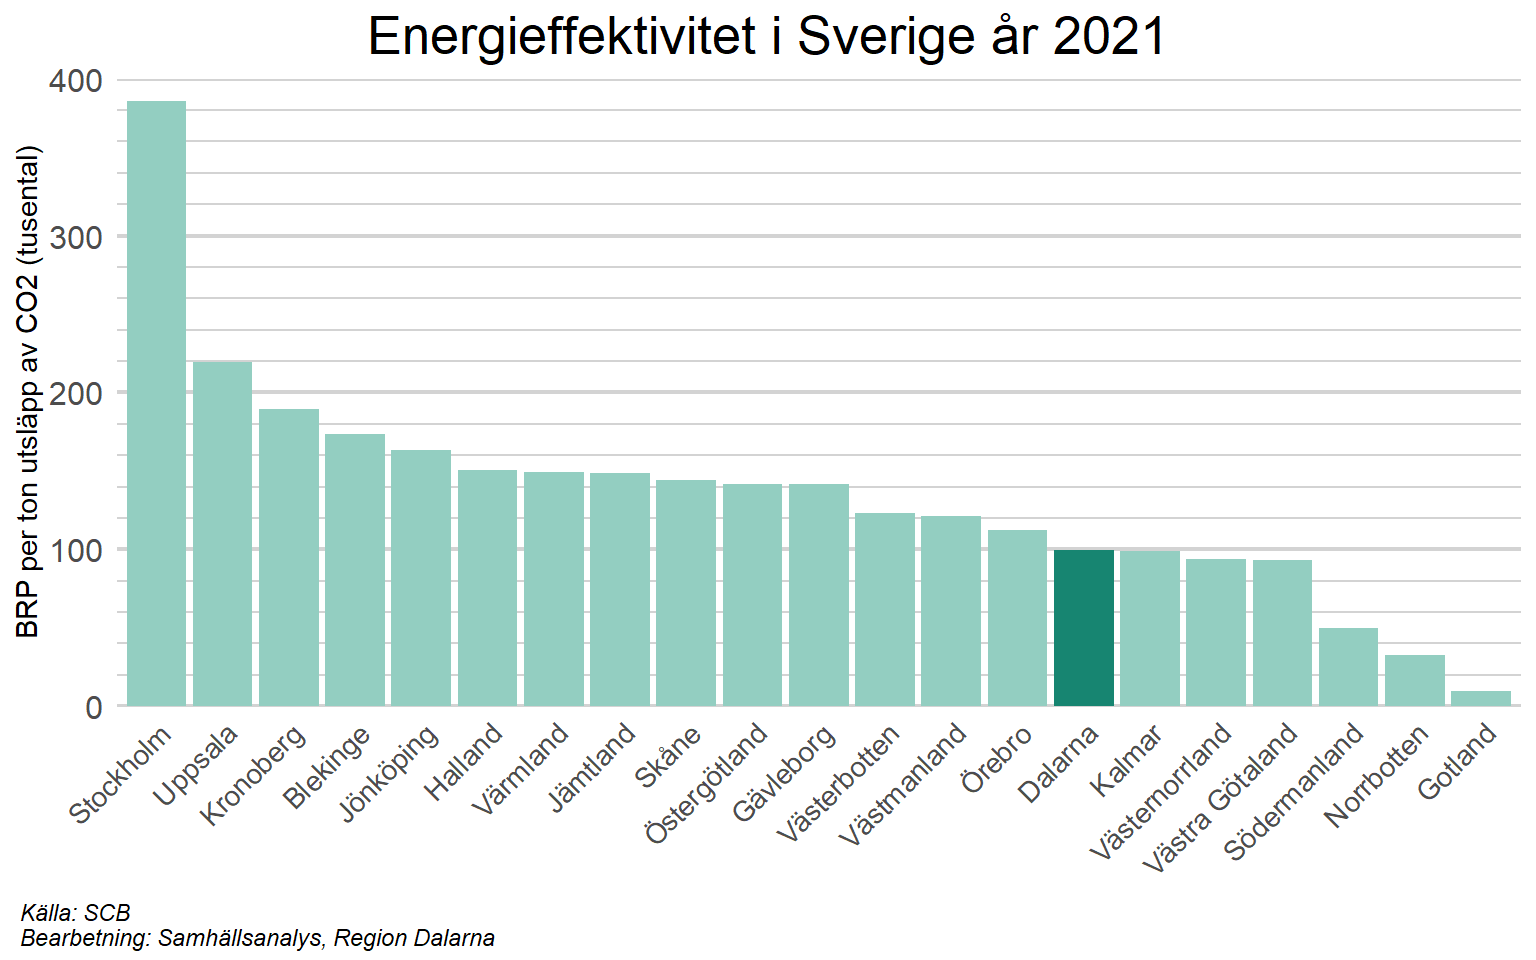
\includegraphics{dalarapport_files/figure-latex/unnamed-chunk-12-1} \end{center}

\hypertarget{andel-kollektivt-resande}{%
\subsection{Andel kollektivt resande}\label{andel-kollektivt-resande}}

På grund av sin utsträckta geografi har Dalarna en utmaning i att
utveckla transportinfrastrukturen ur ett hållbarhetsperspektiv. För att
nå klimat- och energimålen krävs kraftfull teknisk utveckling i
kombination med beteendeförändringar. Kollektivt resande har en central
roll i utvecklandet av en klimatsmart och resurseffektiv, men också mer
jämställd och jämlik mobilitet. Den traditionella kollektivtrafiken
måste kompletteras med nya mobilitetslösningar och tjänster, särskilt
för länets glesa miljöer. Kollektivtrafik är förenat med höga kostnader,
samtidigt som det finns samhällsekonomiska vinster. För att klara
omställningen krävs mod att ställa olika kostnader mot varandra. Det
kollektiva resandet behöver öka.

Här redovisas två olika diagram som indikatorer för kollektivt resande i
Dalarna: resor per invånare samt marknadsandel för kollektivtrafik i
länet. För resor/invånare syns att det kollektiva resandet har legat på
en stabil nivå kring 35 resor per person från 2013 fram till utbrottet
av Covid-19 i Sverige och Dalarna. I det som förmodligen är en
konsekvens av pandemin syns en nedgång i det kollektiva resandet under
2020. Marknadsandelen för kollektivtrafik beräknas som andelen resor med
kollektivtrafik (linjelagd buss, spårvagn, tunnelbana, pendeltåg, tåg
och båt) och taxi av det totala antalet resor med Kollektivtrafik, taxi,
bil (förare och passagerare) samt moped/MC. Även här bryts uppgången i
en förmodad pandemieffekt efter ett antal år av ökande marknadsandel för
kollektivtrafiken.

\begin{center}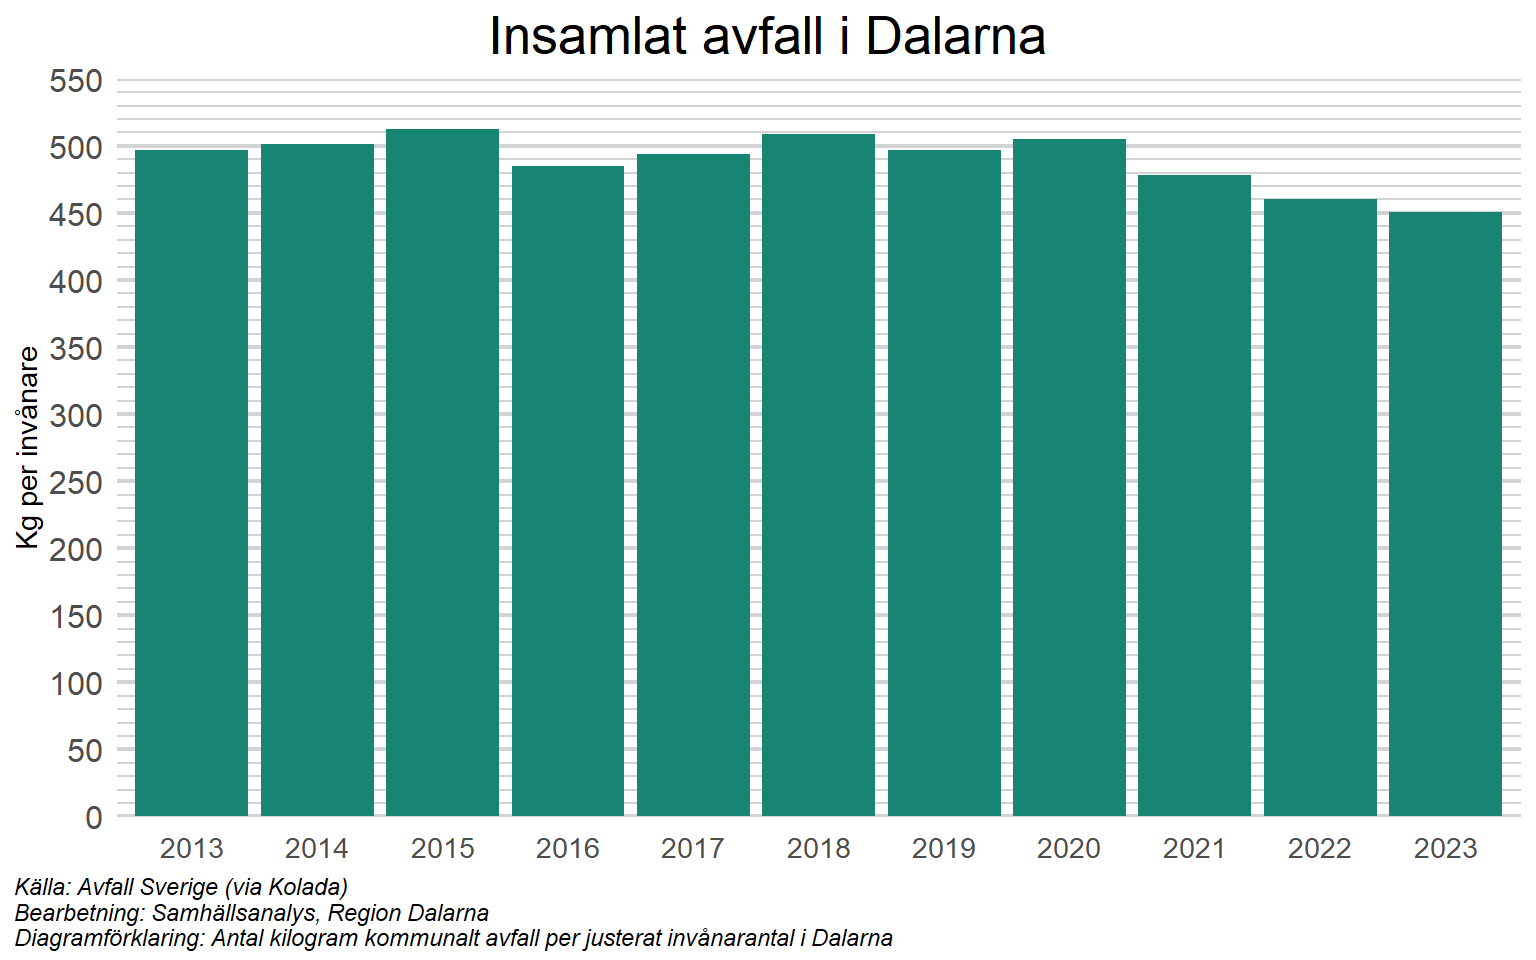
\includegraphics{dalarapport_files/figure-latex/unnamed-chunk-14-1} \end{center}

\begin{center}\includegraphics{dalarapport_files/figure-latex/unnamed-chunk-14-2} \end{center}

\hypertarget{sjuxe4lvfuxf6rsuxf6rjningsgrad-av-energi-och-livsmedel}{%
\subsection{Självförsörjningsgrad av energi och
livsmedel}\label{sjuxe4lvfuxf6rsuxf6rjningsgrad-av-energi-och-livsmedel}}

För att klara utmaningarna med ett förändrat klimat behöver samhället
planera för olika belastningar i form av nederbörd, torka, vind,
insekts- och svampangrepp på grödor och skog, höga temperaturer med
mera. Här spelar god samhällsplanering på regional och kommunal nivå en
viktig roll. Samhällets beredskap behöver utvecklas för att möta de
olika typer av risker som nu ökar till följd av förändringar i klimatet.
En lokal och hållbar livsmedelsproduktion i Dalarna är viktig för såväl
ökad självförsörjningsgrad som för biologisk mångfald. En lokal och
hållbar livsmedelsproduktion i Dalarna är viktig för såväl ökad
självförsörjningsgrad som för biologisk mångfald.

Det första diagrammet visar ett teoretiskt mått på självförsörjning av
livsmedel i länet där producerat livsmedel inom fem kategorier (fårkött,
griskött, matpotatis, mjölkprodukter samt nötkött) visas som en andel av
det som har konsumerats inom samma kategorier i länet. Diagrammet visar
tydligt att befolkningen i Dalarna konsumerar mer inom samtliga dessa
kategorier jämfört med det som produceras i länet.

Det andra diagrammet visar ett teroretiskt mått på självförsöjning av
energi i Dalarna där den totala elproduktionen i länet visas som en
andel av den total elförbrukningen. Diagrammet visar en positiv trend
för självförsörjningsgraden av energi, en trend som drivs både av en
ökande produktion samt en minskande konsumtion.

\begin{center}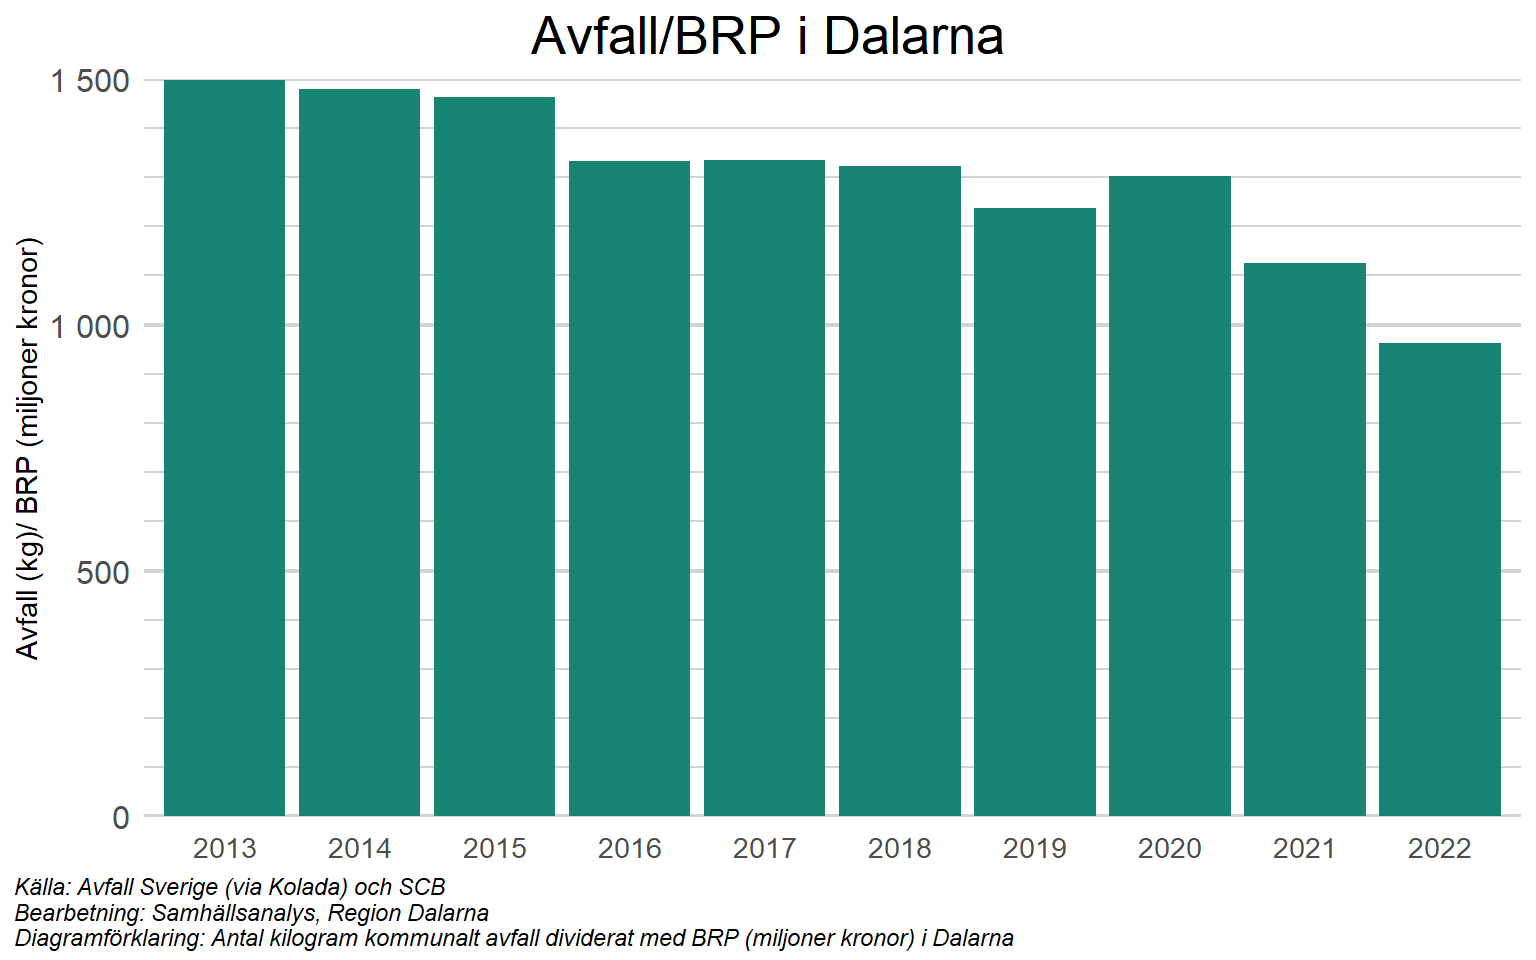
\includegraphics{dalarapport_files/figure-latex/unnamed-chunk-16-1} \end{center}

\begin{center}\includegraphics{dalarapport_files/figure-latex/unnamed-chunk-16-2} \end{center}

\hypertarget{andel-hektar-formellt-skyddad-produktiv-skogsmark}{%
\subsection{Andel hektar formellt skyddad produktiv
skogsmark}\label{andel-hektar-formellt-skyddad-produktiv-skogsmark}}

Regeringen har fattat beslut om Sveriges första nationella skogsprogram
och i Dalastrategin omnämns skogsbruket som en av länets viktiga
näringar. Skogen påverkas också av klimatförändringarna och skötsel och
brukande behöver anpassas därefter. I diagrammen nedan redovisas
utvecklingen för skyddad produktiv skogsmark i Dalarnas län mellan 2018
och 2020. Arealen skyddad skogsmark i länet har minskat något från
116500 hektar till 115400 hektar. Procentuellt var 6.1 procent av den
produktiva skogsmarken i Dalarnas län skyddad 2018 och samma siffra för
2020 var 5.9 procent.

\begin{center}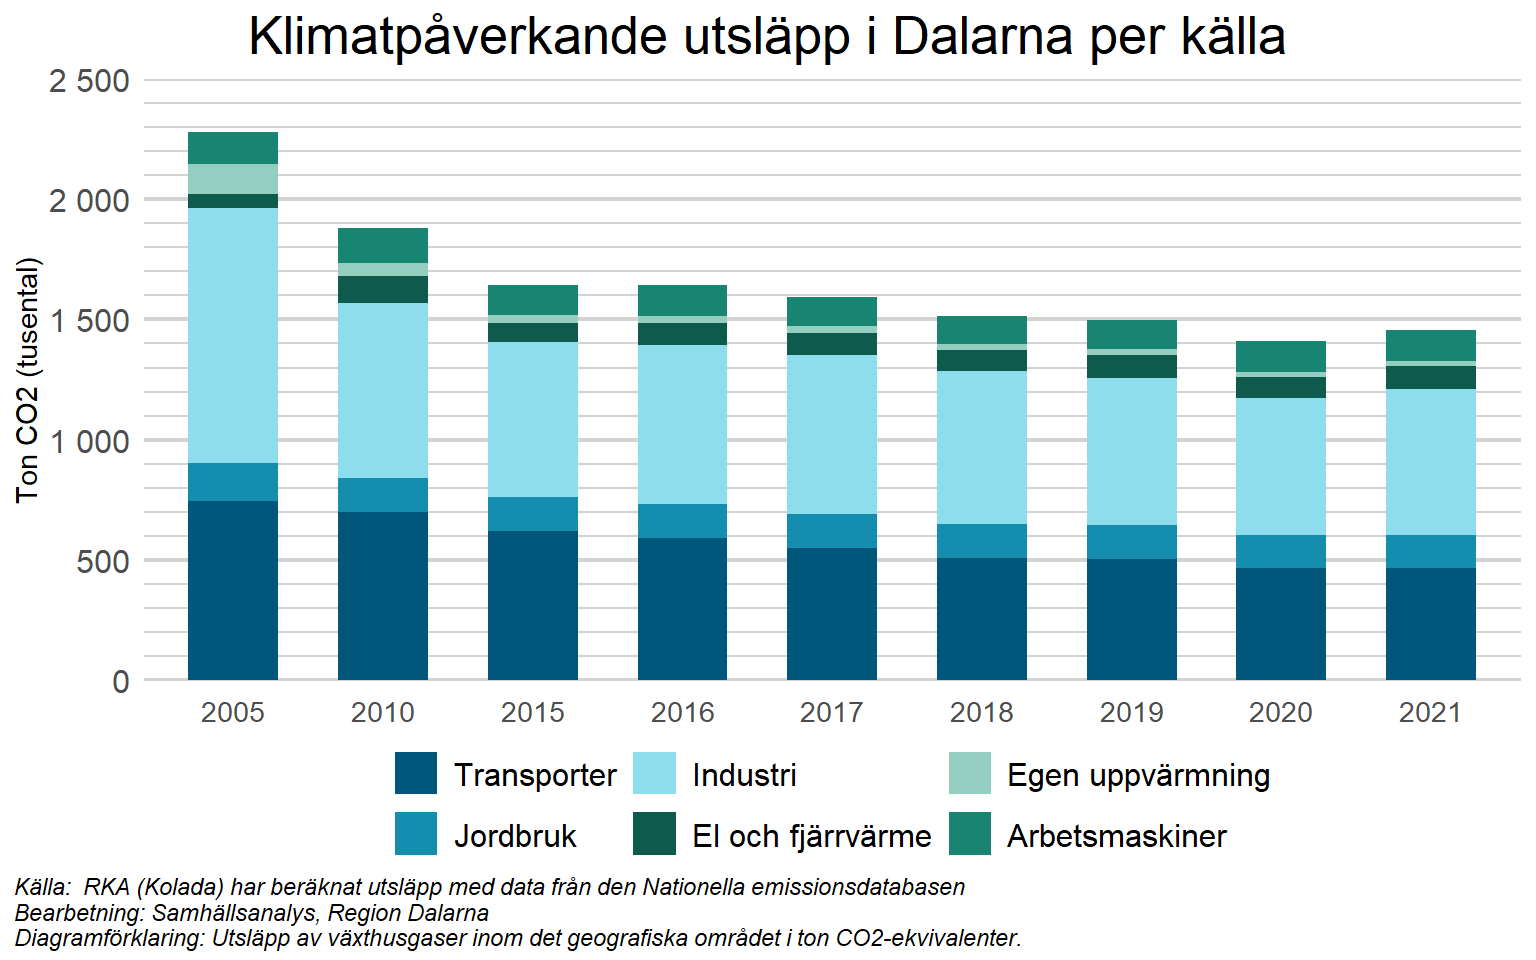
\includegraphics{dalarapport_files/figure-latex/unnamed-chunk-18-1} \end{center}

\begin{center}\includegraphics{dalarapport_files/figure-latex/unnamed-chunk-18-2} \end{center}

\hypertarget{arealen-betesmark-och-areal-med-suxe4rskilt-huxf6ga-biologiska-vuxe4rden}{%
\subsection{Arealen betesmark och areal med särskilt höga biologiska
värden}\label{arealen-betesmark-och-areal-med-suxe4rskilt-huxf6ga-biologiska-vuxe4rden}}

Biologisk mångfald och väl fungerande ekosystem är en förutsättning för
allt liv på jorden. Det är också en bas för goda livsmiljöer både för
Dalarnas invånare och för Dalarnas näringsliv. Ekosystemen behöver
förvaltas så att de fortsatt kan bidra med många olika funktioner
samtidigt. Samhället vinner på aktiva och hållbara näringar och
mångfunktionella landskap där natur- och kulturvärden tillvaratas. Grön
infrastruktur är ekologiskt funktionella nätverk av livsmiljöer och
naturområden som utformas, brukas och förvaltas så att den biologiska
mångfalden bevaras och därmed främjar de för samhället så viktiga
ekosystemtjänsterna.

I diagrammet nedan redovisas utvecklingen för arealen betesmark i
Dalarnas län mellan 2011 och 2020. Arealen har under denna period
minskat från 11908 till 10526 hektar. Denna negativa trend går också
emot den nationella trenden, där arealen betesmark har ökat något i
riket som helhet.

\begin{center}\includegraphics{dalarapport_files/figure-latex/unnamed-chunk-20-1} \end{center}

\hypertarget{ett-konkurrenskraftigt-dalarna}{%
\section{Ett konkurrenskraftigt
Dalarna}\label{ett-konkurrenskraftigt-dalarna}}

I ett konkurrenskraftigt Dalarna är näringslivet livskraftigt och bidrar
till hållbar tillväxt. En väl utvecklad och hållbar infrastruktur skapar
värden för näringsliv, boende och besökare. Det är ett Dalarna där allas
kunskaper och kompetenser tas tillvara och där individer, näringsliv,
offentlig sektor och civilsamhälle utvecklas tillsammans, i samspel med
omvärlden. Det är också ett nyskapande Dalarna där utmaningsdriven
innovation bidrar till ett gott samhälle och hållbar tillväxt.

Den ekonomiska dimensionen av hållbarhet i det regionala
utvecklingsarbetet handlar om att skapa konkurrenskraft och
sysselsättning vilket uppnås genom att använda, hushålla med och förädla
idéer och resurser, på ett miljömässigt och socialt hållbart sätt. Med
ett cirkulärt system där resurser och värden ständigt återskapas främjas
en ekonomiskt hållbar utveckling.

\hypertarget{representation-i-chefspositioner}{%
\subsection{Representation i
chefspositioner}\label{representation-i-chefspositioner}}

Kvinnors och mäns jämställda medverkan och inflytande i näringslivet, på
arbetsmarknaden och i innovationsarbete är och blir en alltmer kritisk
tillväxtfaktor. Konkurrenskraften stärks om kompetenser från olika
grupper oavsett ålder, kön eller bakgrund tas tillvara. En viktig
indikator inom detta område är representation på arbetsmkarnaden,
speciellt i chefspositioner. För 2019 ser vi att det fanns en
överrepresentation av män i chefspositioner på arbetsmarknaden. Kvinnor
och utrikes födda var däremot underrepresenterade.

\begin{center}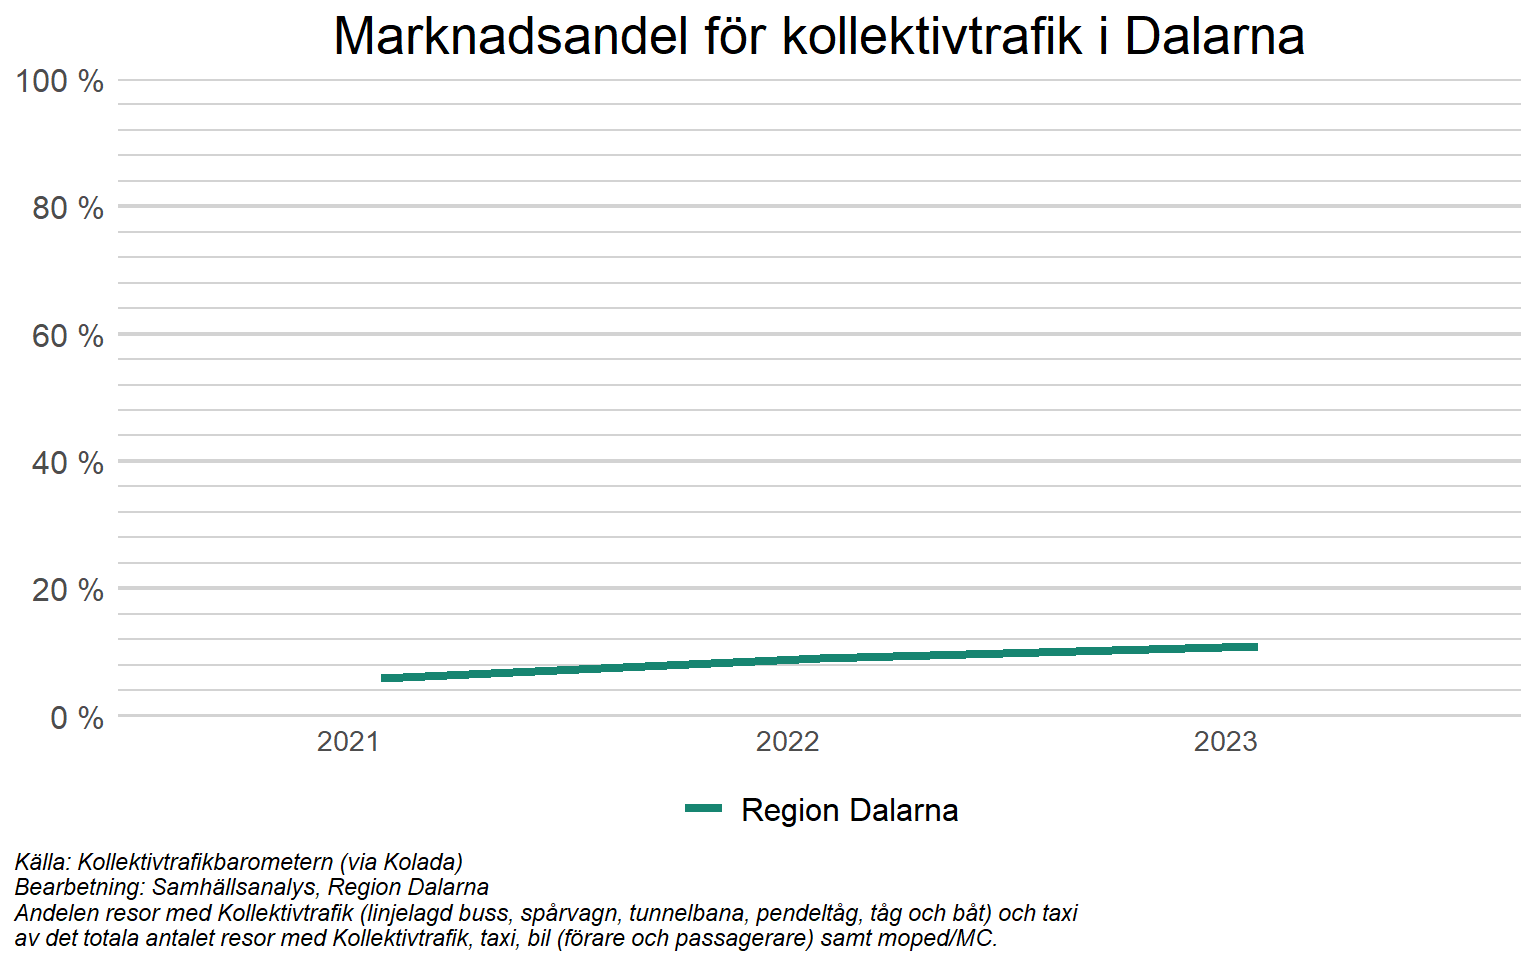
\includegraphics{dalarapport_files/figure-latex/unnamed-chunk-22-1} \end{center}

\hypertarget{ginikoefficient}{%
\subsection{Ginikoefficient}\label{ginikoefficient}}

I Dalastrategin lyfts ekonomiska klyftor som en framtidsutmaning för
länet. För att redovisa ojämnheten i inkomstfördelningen används
gini-koefficienten. Ett högt värde på koefficienten visar på större
ojämnhet. Här redovisas ginikoefficienten avseende disponibel inkomst
per konsumtionsenhet. Konsumtionsenhet avser ett viktsystem där
konsumtionen är relaterad till hushållets sammansättning. Den disponibla
inkomsten divideras med den konsumtionsvikt som gäller för hushållet.

För Dalarnas räkning har ginikoefficienten ökat något från 2011 till
2020, vilket visar på en ökad ekonomisk ojämnhet i länet, med en
toppnotering 2019. Ginikoefficienten för länet ligger under
koefficienten för riket i samtliga år förutom 2019. 2019 avviker dock så
skarpt från den generella trenden för ginikoefficienten att det årets
notering ska betraktas med försiktighet. Ökningen från 2011 och framåt
är dock tydlig även om man bortser från 2019.

\begin{center}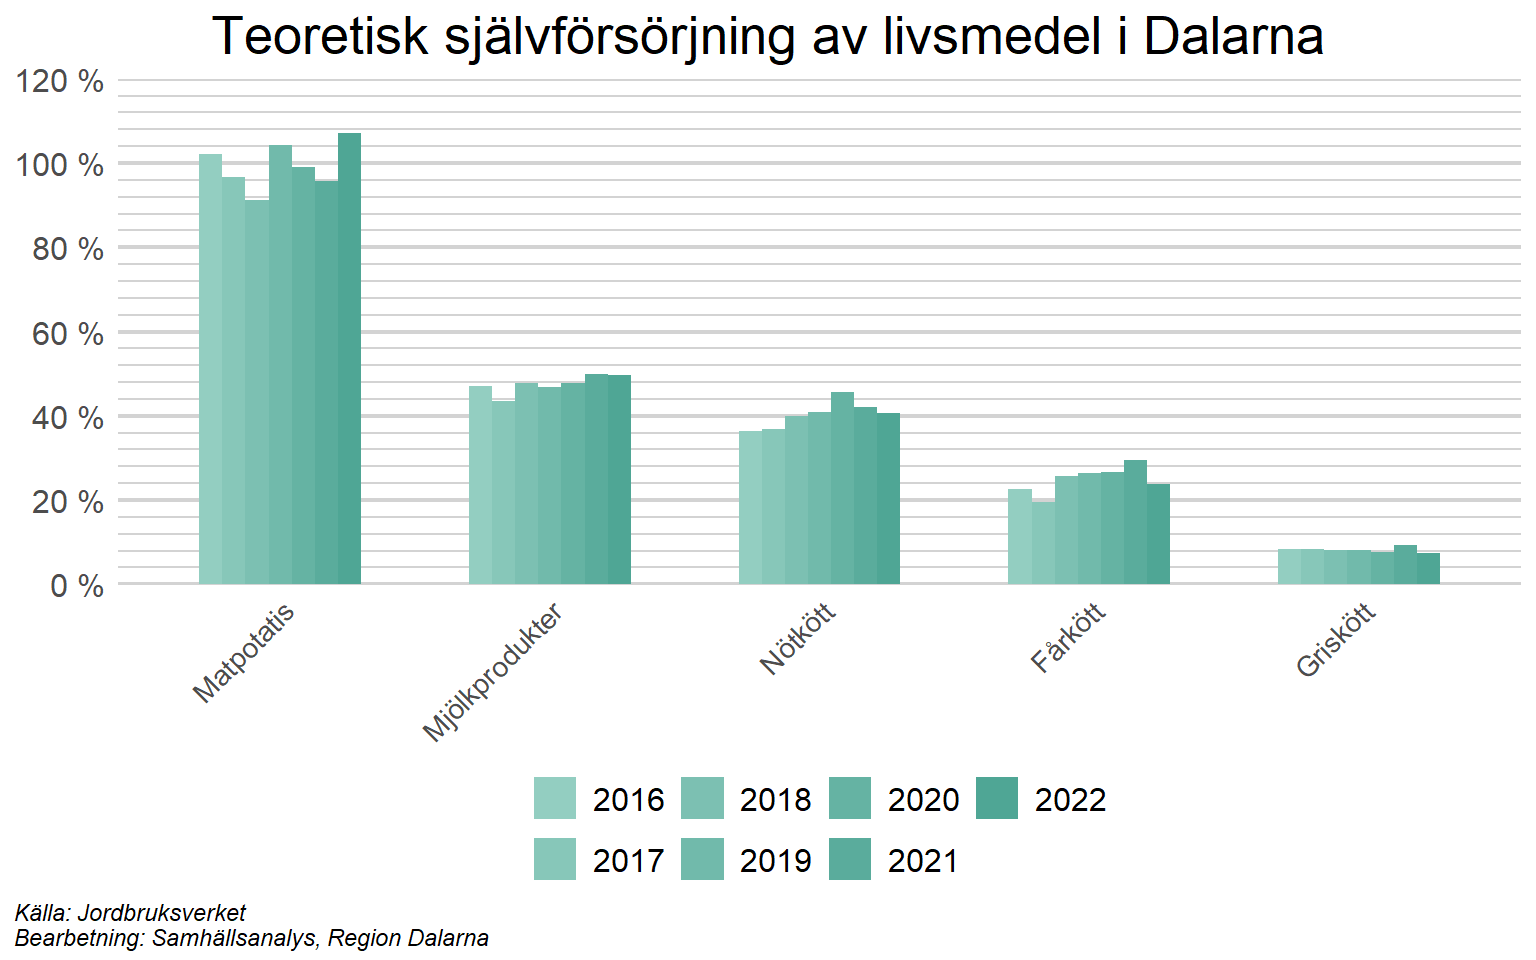
\includegraphics{dalarapport_files/figure-latex/unnamed-chunk-24-1} \end{center}

\hypertarget{internationaliseringsgrad}{%
\subsection{Internationaliseringsgrad}\label{internationaliseringsgrad}}

Dalarna är beroende av omvärlden. Internationell samverkan behövs både
för att möta samhällsutmaningar och för att ta vara på möjligheter till
import, investeringar och export av våra företags varor och tjänster. I
länet finns världsledande företag i olika storlek som deltar i globala
värdekedjor, en del av de mindre utsätts för global konkurrens trots att
de bara eller främst levererar till sin regionala storkund.

En indikator som används för att följa utvecklingen inom detta område är
internationalisering. Internationalisering är ett komplext koncept och
kan bestå av flera olika delar (exempelvis handel, arbetsmarknad och
turism). För uppföljningen av denna indikator används Tillväxtverkets
regionala internationaliseringsindex som är ett sätt att illustrera hur
internationellt integrerade olika regioner är baserat på ett antal olika
variabler. Indexet gör det möjligt att följa hur internationaliseringen
utvecklas över tid i olika regioner (län).

För 2020 ligger Dalarna i mittenskiktet av svenska regioner för
internationalisering. Den region som presterar bäst är Västra
Götalandsregionen och alla andra regioner sätts i relation till den
regionen. Dalarna presterar bättre än de andra regionerna som inkluderas
i Norra Mellansverige (Gävleborg och Värmland). Resultatet för Dalarna
är till viss del ett resultat av att länet presterar bra på delindexet
för turism där länet hamnar på en tredje plats bakom Norrbotten och
Jämtland.

När det kommer till utveckling över tid har Dalarna däremot presterat
sämre än genomsnittet för Sveriges regioner under perioden från
2016-2020.

\begin{center}\includegraphics{dalarapport_files/figure-latex/unnamed-chunk-26-1} \end{center}

\begin{center}\includegraphics{dalarapport_files/figure-latex/unnamed-chunk-26-2} \end{center}

\hypertarget{nyfuxf6retagande}{%
\subsection{Nyföretagande}\label{nyfuxf6retagande}}

För ekonomins och samhällets förnyelse är entreprenörskap en avgörande
faktor. Dalarna behöver fler, och olika typer av entreprenörer och en av
prioriteringarna i Dalastrategin är att främja entreprenörskap och
företagande. Denna indikator mäter antalet nystartade företag i
geografin. Antalet nystartade företag per år i Dalarna har ökat över tid
där toppnoteringen nåddes 2020 med 1744 stycken. År 2007 gjordes en
större förändring i statistiken över nystartade företag vilket kan
förklara den skarpa förändringen från 2006 till 2007.

\begin{center}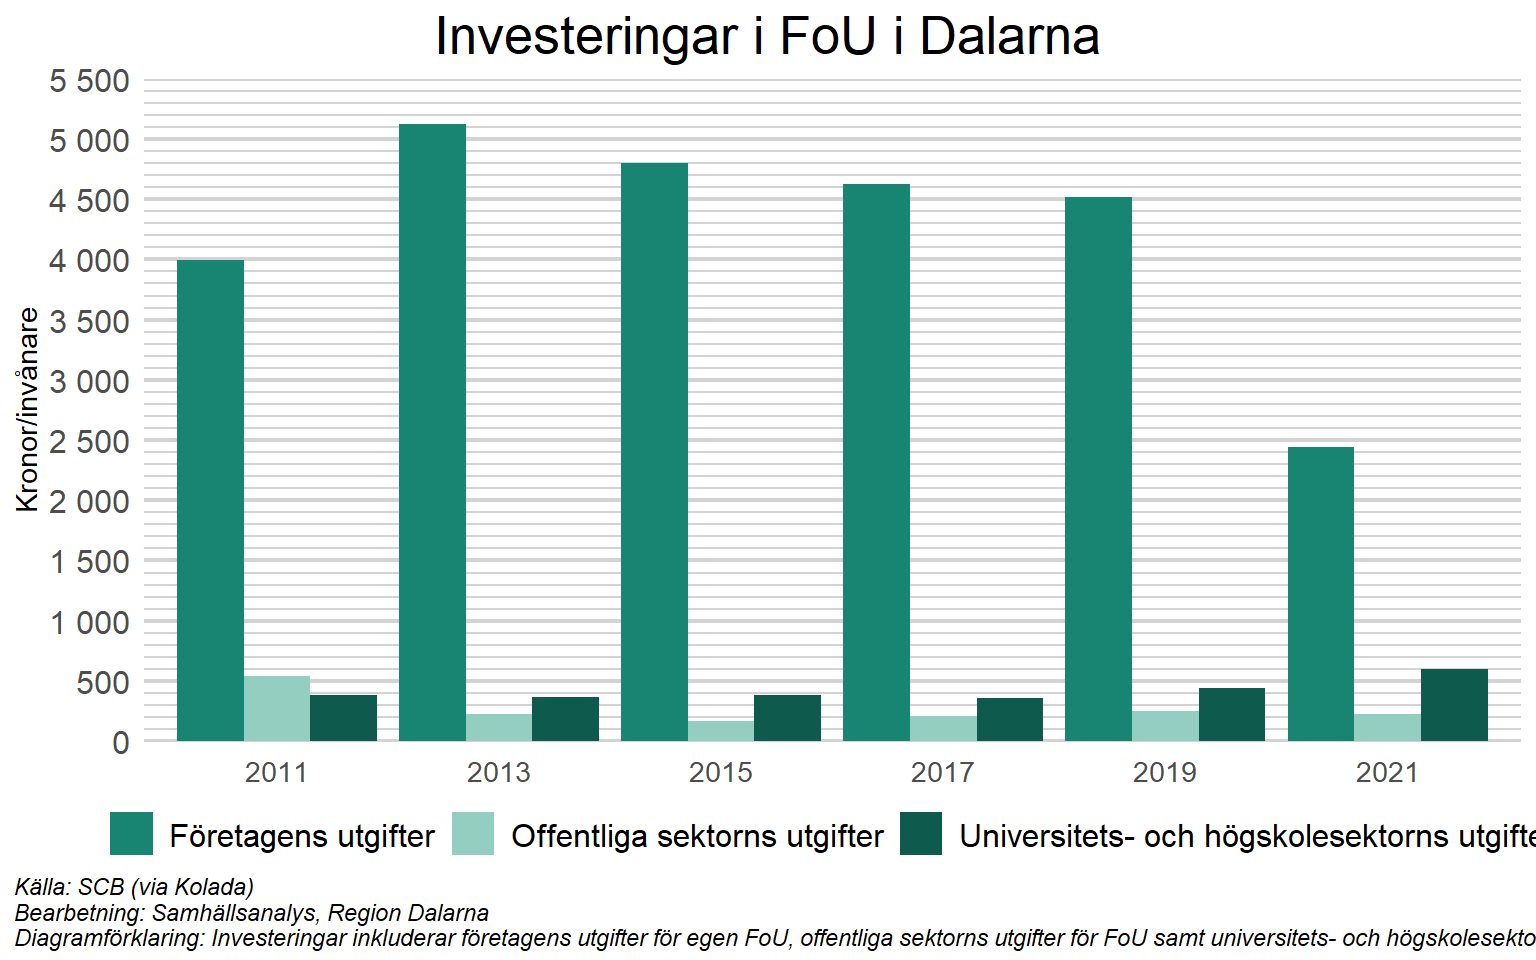
\includegraphics{dalarapport_files/figure-latex/unnamed-chunk-28-1} \end{center}

\hypertarget{matchningsgrad}{%
\subsection{Matchningsgrad}\label{matchningsgrad}}

En förbättrad matchning mellan arbetsmarknadens behov och arbetskraftens
kompetens är nödvändig. Bland annat handlar det om att få till en bättre
samverkan mellan utbildningsanordnare, branscher, näringsliv,
civilsamhället och myndigheter samt över kommun- och länsgränser.
Matchningsindikatorn följer upp hur väl Dalarna lyckas med ambitionen om
bättre matchning.

Matchningsgrad visar andelen anställda som arbetar i yrken som stämmer
väl överens med deras utbildning. För att detta ska gälla ska det dels
finnas en stark överensstämmelse mellan utbildningens och yrkets
ämnesinriktning (t.ex. teknikutbildning -- teknikyrke) och dels ska
utbildningsnivån vara rätt i förhållande till vad yrket kräver.
Matchningsgraden i Dalarna är något högre för kvinnor än för män. För
kvinnor ligger matchningsgraden 2019 på 69,4 procent. För män var
motsvarande mått 67,9 procent. Matchningsgraden för båda dessa grupper
har sjunkit under perioden 2015-2019 och låg i det sista året under
perioden på 68,6 procent.

\begin{center}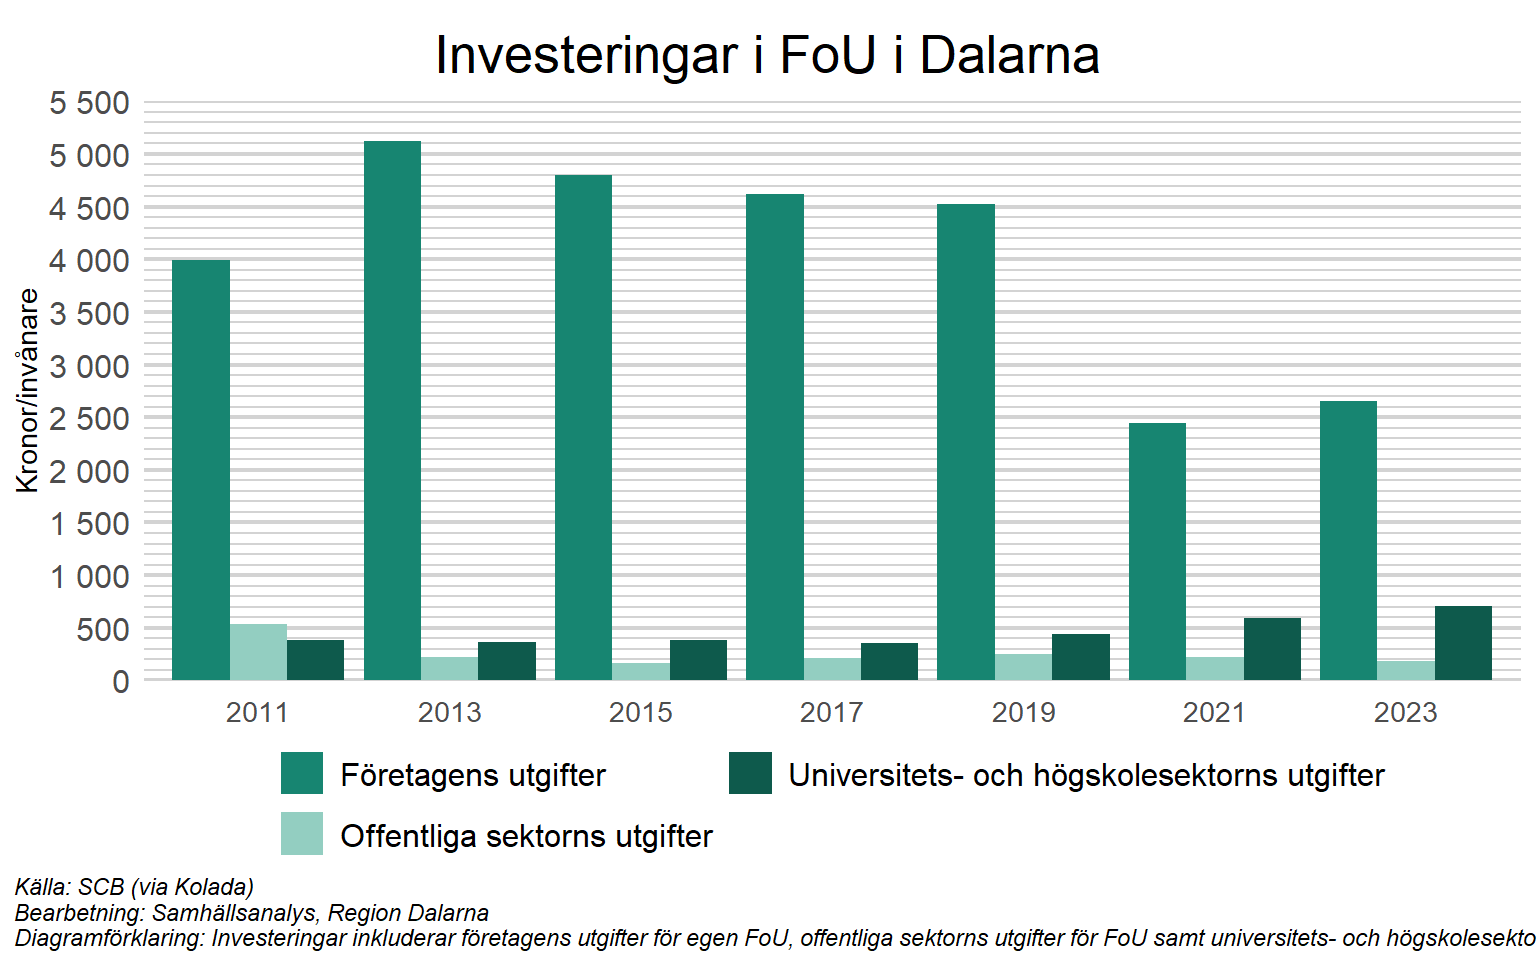
\includegraphics{dalarapport_files/figure-latex/unnamed-chunk-30-1} \end{center}

\hypertarget{andel-sysselsatta}{%
\subsection{Andel sysselsatta}\label{andel-sysselsatta}}

Dalastrategin slår fast att sysselsättningsgraden i länet behöver öka
och skillnader i denna mellan grupper behöver minska. Detta mäts genom
en indikator för förvärvsarbetande i länet uppdelat på kön. I första
året för den inkluderade tidsperioden, 2013, räknades 77,1 procent av
kvinnorna i länet som förvärvsarbetande. Motsvarande siffra för männen i
Dalarna var 79,9 procent. Gapet mellan kvinnor och män var därmed knappt
3 procent. Utvecklingen inom båda grupperna har varit positiv. 2020 var
79,2 procent av kvinnorna förvärvsarbetande och motsvarande siffra för
männen i länet var 81 procent. Gapet mellan dessa grupper har därmed
krympt till knappt 2 procent (1,8). Totalt sett har andelen
förvärvsarbetande i Dalarna ökat från 78,6 till 80,1 procent.

\begin{center}\includegraphics{dalarapport_files/figure-latex/unnamed-chunk-32-1} \end{center}

\hypertarget{luxe5ngtidsarbetsluxf6shet}{%
\subsection{Långtidsarbetslöshet}\label{luxe5ngtidsarbetsluxf6shet}}

En annan indikator för att följa sysselsättningen i länet är andelen
långtidsarbetslösa. Som långtidsarbetslös räknas den som har varit öppet
arbetslösa eller i program med aktivitetsstöd i minst sex månader. Om
utvecklingen för andelen förvärsarbetande kan beskrivas som positiv och
i rätt riktningen så kan inte samma sak sägas om denna indikator. 2014
noterades 2,9 procent av länets befolkning som långtidsarbetslösa. 2021
var motsvarande siffra 3,9 procent. För kvinnor har andelen
långtidsarbetslösa ökat från 2,6 procent till 3,7 procent under
tidsperioden. För den manliga befolkningen i länet är motsvarande
förändring också en ökning, från 3,1 procent till 4 procent år 2021.

\begin{center}\includegraphics{dalarapport_files/figure-latex/unnamed-chunk-34-1} \end{center}

\hypertarget{andel-unga-som-inom-fyra-uxe5r-fullfuxf6ljer-gymnasieutbildning}{%
\subsection{Andel unga som inom fyra år fullföljer
gymnasieutbildning}\label{andel-unga-som-inom-fyra-uxe5r-fullfuxf6ljer-gymnasieutbildning}}

Kunskap ger människor möjlighet att växa och påverka sin livssituation.
Tillgång till bildning, kunskap och kompetens är avgörande för såväl
utvecklingen av samhället, god välfärd och tillväxt i näringslivet. När
arbetsgivare inte hittar rätt kompetens hämmas den ekonomiska
utvecklingen. Samtidigt försvagas den sociala hållbarheten när människor
ställs utanför arbetsmarknaden. Låga utbildningsnivåer är en utmaning i
stora delar av Dalarna. Ambitionen i Dalastrategin är därmed att fler
ska klara en gymnasiexamen för att kunna etablera sig på
arbetsmarknaden.

Denna indikator mäter andelen gymnasiestudenter som har fullföljt sin
utbildning inom fyra år i Dalarna. Utvecklingen över tid från 2011 till
2017 är negativ. Av studenterna som började läsa på gymnasiet i Dalarna
2011 är det 72,6 procent som inom fyra år fullföljde sin utbildning med
examen. Motsvarande mått för 2017 är 69,9 procent och därmed en
minskning med 2,7 procent.

\begin{center}\includegraphics{dalarapport_files/figure-latex/unnamed-chunk-36-1} \end{center}

\hypertarget{andel-huxf6gskoleutbildade-i-befolkningen}{%
\subsection{Andel högskoleutbildade i
befolkningen}\label{andel-huxf6gskoleutbildade-i-befolkningen}}

Med en alltmer kunskapsintensiv ekonomi ökar också behovet av
eftergymnasialt utbildade. Dalastrategin lyfter betydelsen av en stark
regional högskola med närvaro i hela länet. Även andra utbildningsformer
såsom folkhögskolor, yrkesvux och yrkeshögskolor bidrar till stärkt
kompetensförsörjning i form av såväl bredd som spets. Indikatorn
innefattar invånare med eftergymnasial utbildning mellan 25 och 64 år.
Med eftergymnasial utbildning avses eftergymnasial utbildning kortare än
3 år, längre än 3 år samt forskarutbildning.

Indikatorn visar på en positiv utveckling över tid där andelen med
eftergymnasial utbildning har ökat från 31,2 procent till 34,2 procent
mellan 2013 och 2020. Det finns också en uppenbar skillnad mellan män
och kvinnors utbildningsnivå. 2020 hade 41,7 procent av kvinnorna i
Dalarna någon form av eftergymnasial utbildning. Motsvarande siffra för
männen i Dalarna var avsveärt lägre på 27 procent.

\begin{center}\includegraphics{dalarapport_files/figure-latex/unnamed-chunk-38-1} \end{center}

\hypertarget{etableringstid-fuxf6r-nyanluxe4nda}{%
\subsection{Etableringstid för
nyanlända}\label{etableringstid-fuxf6r-nyanluxe4nda}}

Invandringen är en del i lösningen för god kompetensförsörjning. Dalarna
har haft en relativt stor inflyttning av utomeuropeiskt födda under
senare år. Då många nyanlända är i arbetsför ålder är de ett viktigt
tillskott till arbetskraften. Denna indikator är ett mått på i vilken
utsträckning nyanlända etablerar sig på arbetsmarknaden i Dalarna.

Andelen etablerade på arbetsmarknaden ökar efter vistelsetid i landet.
Bland gruppen nyanlända som har vistats i Sverige en kortare period
(exempelvis upp till ett år) är andelen förvärvsarbetande avsevärt lägre
jämfört med nyanlända som har vistats i landet en längre tid. För det
senaste året i period, 2020, hade knappt 37 procent av nyanlända med
vistelsetid under ett år etablerat sig på arbetsmarknaden. Andelen
etablerade på arbetsmarknaden stiger sedan alltmer efter vistelsetid och
för samma år var det lite drygt 71 procent i gruppen som vistats i
Sverige i tio år eller mer som etablerat sig.

Ytterliggare en trend är att det över tid går snabbare för nyanlända att
etablera sig på arbetsmarknaden. Från 2015 till 2020 har andelen
etablerade på arbetsmarknaden med kort vistelsetid (under 1 år) ökat
från 14 procent till knappt 37 procent. Det existerar också tydliga
skillnader mellan män och kvinnors etablering där en högre andel kvinnor
lyckas etablera sig på arbetsmarknaden tidigare än männen. Skillnaderna
mellan könen blir dock mindre över tid och i gruppen som har vistats i
landet i minst tio år skiljer det endast 0,1 procent.

\begin{center}\includegraphics{dalarapport_files/figure-latex/unnamed-chunk-40-1} \end{center}

\begin{center}\includegraphics{dalarapport_files/figure-latex/unnamed-chunk-40-2} \end{center}

\begin{center}\includegraphics{dalarapport_files/figure-latex/unnamed-chunk-40-3} \end{center}

\begin{center}\includegraphics{dalarapport_files/figure-latex/unnamed-chunk-40-4} \end{center}

\hypertarget{investeringar-i-fou}{%
\subsection{Investeringar i FoU}\label{investeringar-i-fou}}

För att lösa dagens och morgondagens samhällsutmaningar och för
utveckling och konkurrenskraft krävs ökad innovationskraft. Individers,
företags, organisationers och offentlig sektors innovationsförmåga
påverkar platsers utvecklingskraft och möjligheter till omställning.
Denna indikator mäter investeringar i forsking och utveckling i länet.
Det bör dock noteras att innovation och forskning är ett synnerligen
svårt område att mäta och att denna indikator främst ger en bild av hur
stora resurser som investeras i länet.

Under tidsperioden från 2011 till 2019 ser vi en ökning i utgifter mätt
i kronor per invånare i länet, från drygt 4900 kronor till drygt 5200
kronor per invånare. Investeringar sker främst bland företag med mindre
bidrag från den offentliga sektorn samt universitet- och
högskolesektorn. I ett nationellt perspektiv ser vi att Dalarna hamnar
på den nedre halvan. Östergötland, som har den högsta noteringen för
utgifter inom forskning och utveckling, har knappt sex gånger högre
utgifter per invånare jämfört med Dalarna.

\begin{center}\includegraphics{dalarapport_files/figure-latex/unnamed-chunk-42-1} \end{center}

\begin{center}\includegraphics{dalarapport_files/figure-latex/unnamed-chunk-42-2} \end{center}

\begin{center}\includegraphics{dalarapport_files/figure-latex/unnamed-chunk-42-3} \end{center}

\hypertarget{ett-sammanhuxe5llet-dalarna}{%
\section{Ett sammanhållet Dalarna}\label{ett-sammanhuxe5llet-dalarna}}

I ett sammanhållet Dalarna finns goda livsmiljöer som skapar en känsla
av närhet. Det är ett Dalarna fyllt av engagemang, där människor
upplever delaktighet och tillsammans bidrar till en hållbar utveckling.
Det är ett inkluderande, jämställt, och jämlikt Dalarna där människor
mår bra och där alla ges möjlighet att utvecklas.

Den sociala dimensionen av hållbarhet i det regionala utvecklingsarbetet
handlar om att alla människor, utifrån sina behov och förutsättningar,
ges likvärdiga möjligheter att delta i samhällsutvecklingen. Ju fler som
känner sig delaktiga, desto mer utveckling kan åstadkommas.

\hypertarget{truxe5ngboddhet}{%
\subsection{Trångboddhet}\label{truxe5ngboddhet}}

Goda livsmiljöer som upplevs som trygga och inkluderande är en
förutsättning för att människor ska må bra. Olika platser i Dalarna har
olika utmaningar och möjligheter, bland annat beroende på om det är
platser med växande eller krympande befolkningsunderlag, att möta dessa
behov. Indikatorn trångboddhet relaterar bland annat till prioriteringen
i Dalastrategin om diversifierade boendeformer som i sin tur motverkar
segregation och polarisering.

Antalet trångbodda i Dalarna har ökat under perioden från 2012 till
2020. I början på perioden var det 8812 individer i Dalarna som räknades
som trångbodda enligt norm 2. Åtta år senare hade denna siffra ökat till
13 801 personer. Detta är dock lägre än toppnoteringen 2019 på 14 576
personer och kan vara början på en nedåtgående trend.

\begin{center}\includegraphics{dalarapport_files/figure-latex/unnamed-chunk-44-1} \end{center}

\hypertarget{boendetyper}{%
\subsection{Boendetyper}\label{boendetyper}}

Ytterligare en indikator inom samma område är relaterad till typen av
boende inom länet. Småhus är den dominerande boendeformen i länet med 76
928 hushåll, en ökning från 74 272 hushåll 2012. 15 598 hushåll
inkluderas i gruppen hyresrätt i flerbostadshus medan 1 720 hushåll
återfinns i gruppen flerbostadshus med bostadsrätt.

\begin{center}\includegraphics{dalarapport_files/figure-latex/unnamed-chunk-46-1} \end{center}

\hypertarget{tillguxe5ng-till-service-och-tjuxe4nster}{%
\subsection{Tillgång till service och
tjänster}\label{tillguxe5ng-till-service-och-tjuxe4nster}}

Olika platser i Dalarna har olika utmaningar och möjligheter, bland
annat beroende på om det är platser med växande eller krympande
befolkningsunderlag, att möta dessa behov. Med utgångspunkt, och som
princip för genomförandet, att allt utvecklingsarbete ska vara
platsbaserat ska den geografiska sammanhållningen stärkas och olika
platsers förutsättningar och resurser tas tillvara. För utvecklingskraft
i hela länet är det viktigt att säkra tillgången till service, vård,
fritidsaktiviteter och kultur. Människor behöver ha en god
tillgänglighet till såväl statlig som regional och kommunal service.
Tillgången till service påverkar också människor levnadsvillkor och är
viktigt för en plats attraktivitet.

Den här indikatorn presenterar två olika mått på tillgång till service;
tillgång till grundskola samt tillgång till dagligvarubutik. Tillgång
till grundskola har förbättras under perioden från 2010 till 2020. I
början på perioden hade drygt 69,5 procent av alla invånare mellan 0-16
år en grundskola inom 2km från bostaden. 2020 hade motsvarande siffra
ökat till 71,2 procent. Samma trend existerar inte för tillgång till
dagligvarubutiker. Under samma period har andelen med en dagligvarubutik
inom 2km från bostaden minskat från 66,3 procent till 65,3 procent.

\begin{center}\includegraphics{dalarapport_files/figure-latex/unnamed-chunk-48-1} \end{center}

\hypertarget{deltagande-i-det-civila-samhuxe4llet}{%
\subsection{Deltagande i det civila
samhället}\label{deltagande-i-det-civila-samhuxe4llet}}

Att stärka sammanhållningen och med det den sociala hållbarheten, är
viktigt för Dalarnas utveckling. Ett socialt hållbart samhälle tål
påfrestningar, är anpassningsbart och resilient. Det är människorna i
Dalarna som är regionens främsta resurs -- som individer och del av
familjer, andra gemenskaper, organisationer och företag. Människors
känsla av sammanhang och delaktighet är centrala delar i det som ibland
benämns socialt kapital.

Denna indikator visar andelen (\%) invånare 18-80 år med lågt socialt
deltagande. Indikatorn ingår även i BRP+, regionernas uppföljningssystem
för hållbar utveckling och livskvalitet.

Perioden från 2007 till 2020 i Dalarna uppvisar ett antal olika trender
och mönster. Från början på perioden genom 2015 steg andelen invånare
mellan 18-80 år som uppgav att man deltagit i högst en aktivitet. Från
2016 och framåt sjunker andelen snabbt och är tillbaka på samma eller en
lägre nivå än 2007. För 2020 uppger kvinnor och män nästan samma nivå av
låg delaktighetet med 21 respektive 22 procent. För den manliga delen av
befolkningen är detta en stor förbättring jämfört med fem år tidigare då
andelen med lågt socialt deltagande uppgick till hela 29 procent.

\begin{center}\includegraphics{dalarapport_files/figure-latex/unnamed-chunk-50-1} \end{center}

\hypertarget{andel-av-hushuxe5ll-som-har-tillguxe5ng-till-bredband}{%
\subsection{Andel av hushåll som har tillgång till
bredband}\label{andel-av-hushuxe5ll-som-har-tillguxe5ng-till-bredband}}

Tillgång till en snabb och robust digital infrastruktur är en
grundförutsättning för att bo och verka i hela Dalarna. Fysiska och
digitala mötesplatser gör att vi når både varandra och omvärlden. En av
utmaningarna för Dalarna är en ojämnt fördelad digital infrastruktur.
Att stärka och tillgängliggöra den digitala infrastrukturen för hela
Dalarnas befolkning, oavsett plats, är avgörande för en lyckad
digitalisering av samhället.

I Dalarna har andelen av befolkningen med tillgång till bredband ökat
från drygt 47 procent 2015 till drygt 76 procent 2020. Andelen som
redovisas här har tillgång till bredband om minst 100 Mbit/s och
indikatorn inkluderas även i BRP+, regionernas uppföljningssystem för
hållbar utveckling och livskvalitet.

\begin{center}\includegraphics{dalarapport_files/figure-latex/unnamed-chunk-52-1} \end{center}

\hypertarget{valdeltagande}{%
\subsection{Valdeltagande}\label{valdeltagande}}

Dalastrategin belyser vikten av att den representativa demokratins
institutioner, såsom kommuner, region och myndigheter, är väl fungerande
och uppbär människors tillit som centralt för en levande demokrati.
Valdeltagande inkluderas därmed som en indikator för att följa upp
invånarnas vilja och tro på de demokratiska institutionerna i länet.
Valdeltagande ingår även som en indikator i BRP+, regionernas
uppföljningssystem för hållbar utveckling och livskvalitet.

I Dalarna har valdeltagandet i både kommun-, region- samt riksdagsval
ökat mellan valen 1998 och 2018. 1998 valde drygt 78,4 procent av
invånarna i Dalarna att lägga en röst i kommunvalet. 2018 var
motsvarande drygt 85,4 procent, en ökning med 7 procent. I varje val
under tidsperioden har en högre andel valt att avlägga en röst i
riksdagsvalet än i kommunvalet. Ännu färre väljer att rösta i
landstings/regionvalet som har lägst valdeltagande.

\begin{center}\includegraphics{dalarapport_files/figure-latex/unnamed-chunk-54-1} \end{center}

\begin{center}\includegraphics{dalarapport_files/figure-latex/unnamed-chunk-54-2} \end{center}

\begin{center}\includegraphics{dalarapport_files/figure-latex/unnamed-chunk-54-3} \end{center}

\hypertarget{tillit-till-andra-muxe4nniskor}{%
\subsection{Tillit till andra
människor}\label{tillit-till-andra-muxe4nniskor}}

Det är människorna i Dalarna som är regionens främsta resurs -- som
individer och del av familjer, andra gemenskaper, organisationer och
företag. Människors känsla av sammanhang och delaktighet är centrala
delar i det som ibland benämns socialt kapital. Ett högt socialt kapital
är det kitt som får människor att trivas och är nödvändigt för att
människor ska vilja bidra till samhällsutvecklingen. När människor
känner sig som en del av samhället leder detta ofta också till en hög
tillit till andra människor. Att den representativa demokratins
institutioner, såsom kommuner, region och myndigheter, är väl fungerande
och uppbär människors tillit är centralt för en levande demokrati. En
hög tillit till andra underlättar även möten mellan människor där nya
idéer kan uppstå och utvecklas. Ett samhälle med gott socialt kapital
grundar för ett resilient samhälle, väl rustat att möta förändring och
eventuella kriser.

Indikatorn som presenteras här nedan ger en bild av tillit i Dalarna.
Indikatorn mäter andel (\%) invånare 16-84 år med avsaknad av tillit
till andra och inkluderas även i BRP+, regionernas uppföljningssystem
för hållbar utveckling och livskvalitet. Tidsperioden från 2007 till
2021 visar på en sjunkande (positiv) trend för den här indikatorn. 2007
uppgav 28 procent av respondenterna i Dalarna en avsaknad av tillit till
andra. 2021 var motsvarande siffra 26 procent. En högre andel av kvinnor
uppger en avsaknad av tillit till andra men den positiva utvecklingen
för indikatorn är till stor del en effekt av att andelen kvinnor med
tillit till andra har ökat från 2007 till 2021.

\begin{center}\includegraphics{dalarapport_files/figure-latex/unnamed-chunk-56-1} \end{center}

\hypertarget{andel-invuxe5nare-i-ekonomiskt-utsatta-hushuxe5ll}{%
\subsection{Andel invånare i ekonomiskt utsatta
hushåll}\label{andel-invuxe5nare-i-ekonomiskt-utsatta-hushuxe5ll}}

Ekonomiska klyftor mellan olika grupper i samhället är en utmaning för
både Sverige och Dalarna. Om de socioekonomiska klyftorna blir alltför
stora riskerar de att motverka sammanhållning, tillit och trygghet. Det
riskerar i sin tur att försvaga demokratin, exempelvis genom
systematiska skillnader i valdeltagande, faktiskt eller upplevt
inflytande samt delaktighet och engagemang.

Andel barn som lever i ekonomiskt utsatta hushåll är ett mått på
levnadsstandard som speglar möjligheterna för en av de mest utsatta
grupperna i samhället. Detta mått ingår även i BRP+, regionernas
uppföljningssystem för hållbar utveckling och livskvalitet. Med
ekonomiskt utsatta avses hushåll med låg inkomst eller ekonomiskt
bistånd (tidigare kallat socialbidrag). Med låg inkomst avses lägsta
utgiftsnivå baserad på den socialbidragsnorm, som fastställdes på
1980-talet (med inflationsuppräkningar) och en norm för boendeutgifter.
Om inkomsterna understiger dessa normer definieras detta som låg inkomst
(för mer information om måttet, se Kolada.se).

I diagrammet nedan kan vi notera att andelen unga i ekonomiskt utsatta
hushåll i Dalarnas län låg på lite drygt 11 procent 2020. Det är en
något mindre andel än det var 2010 (12,4 procent) men högre än den
lägsta noteringen i tidsspannet som nåddes 2016 på 10,6 procent. I ett
nationellt perspektiv ser vi att endast tre andra län har en högre andel
ekonomiskt utsatta unga.

\begin{center}\includegraphics{dalarapport_files/figure-latex/unnamed-chunk-58-1} \end{center}

\begin{center}\includegraphics{dalarapport_files/figure-latex/unnamed-chunk-58-2} \end{center}

\hypertarget{andel-unga-som-upplever-att-de-uxe4r-delaktiga-i-sin-kommun}{%
\subsection{Andel unga som upplever att de är delaktiga i sin
kommun}\label{andel-unga-som-upplever-att-de-uxe4r-delaktiga-i-sin-kommun}}

Hållbar utveckling kräver förståelse för och kunskap om framtida
generationers utmaningar och behov. FN:s konvention om barnets
rättigheter, eller barnkonventionen som den ofta kallas, är svensk lag
och syftar till att ge barn oavsett bakgrund rätt att behandlas med
respekt och att få komma till tals. Barn och unga i Dalarna måste ges
möjlighet att ta en aktiv del i samhällsutvecklingen för att målen i
Dalastrategin ska kunna uppnås.

För att kunna följa utvecklingen på det här området inkluderas en
indikator för ungas delaktighet i Dalastrategin. Data för indikatorn
hämtas från ungdomsenkäten LUPP som genomförs vart tredje år. Här
redovisas andelen unga som har angett ganska eller mycket stora
möjligheter att föra fram sina åsikter till dem som bestämmer i
kommunen.

Utvecklingen för denna indikator är sammantaget negativ. På gymnasienivå
är andelen som har svarit att det finns möjligheter till delaktighet
ungefär lika stor 2015 som 2021 (19,8 respektive 19,5 procent) även om
det är en svag minskning. En tydligare trend finns bland
högstadieungdomar där andelen som ser möjligheter till delaktighet har
sjunkit från 23,4 till 19 procent.

\begin{center}\includegraphics{dalarapport_files/figure-latex/unnamed-chunk-60-1} \end{center}

\hypertarget{sjuxe4lvskattad-huxe4lsa}{%
\subsection{Självskattad hälsa}\label{sjuxe4lvskattad-huxe4lsa}}

Folkhälsan varierar hos befolkningen, både i riket och mellan platser i
Dalarnas län. Personer med lägre utbildningsnivå har generellt sett en
sämre hälsa och sämre förutsättningar för en god hälsa än de med högre
utbildningsnivå. Självskattad hälsa är en av de indikatorer som
Folkhälsomyndigheten har valt för att mäta folkhälsan och dess
förutsättningar. Det är även en av indikatorerna som återfinns under
avsnittet för ett sammanhållet Dalarna i Dalastrategin.

För 2021 var det totalt 69 procent av respondenterna i Dalarnas län som
uppgav ett bra eller mycket bra allmänt hälsotillstånd. För tidsperioden
2014-2021 har det allmänna hälsotillståndet i länet varit stabilt runt
68-69 procent utan några större förändringar. Däremot framkommer det att
en något större andel av män upplever ett bättre hälsotillstånd än
kvinnliga respondenter.

I ett nationellt perspektiv ligger alla utom en kommun i Dalarnas län
under riksgenomsnittet. Av befolkningen 16-84 år var det enligt 2021 års
undersökning 74 procent som uppgav att de har en bra eller mycket bra
hälsa. Även på nationell nivå är andelen högre bland män än bland
kvinnor, och högre bland yngre jämfört med äldre. I Älvdalen uppgav 74
procent en god eller mycket bra hälsa och motsvarande siffra för
Smedjebacken var 66 procent.

\begin{center}\includegraphics{dalarapport_files/figure-latex/unnamed-chunk-62-1} \end{center}

\begin{center}\includegraphics{dalarapport_files/figure-latex/unnamed-chunk-62-2} \end{center}

\end{document}
